\chapter{Supplementary Materials: rumi} 


% Section
\section{Protein function prediction scenarios}

In protein function prediction, there are two scenarios in which a computational model can be constructed \citep{Radivojac2013}: (i) given a new protein, the task of a classifier is to find all functional terms that the protein is associated with ("what is the function of this protein?"); and (ii) given a functional term, the task of a classifier is to find all proteins associated with this term ("what are the proteins associated with this function?"). Undoubtably, the two prediction scenarios are related because a perfect predictor of protein function would solve both questions at the same time. However, imperfect predictors may address one question better than the other. For example, a classifier built to address the first question is expected to be accurate in predicting all (or many) functional terms and that prediction scores over all functional terms are comparable. On the other hand, a predictor developed to consider only one functional term at a time need not consider any other term. Such models can perform well even if they just rank all test proteins. In addition to these differences, the two types of models are evaluated in different ways (yet they use the same terminology).

The models that are concerned with predicting function on a previously unseen protein (scenario 1, above) need to devise evaluation metrics to estimate the expected accuracy of a predicted consistent graph $P$ when the experimental (true) annotation of the protein is graph $T$. Alternatively, the models that are concerned with ranking the proteins according to their likelihood to be associated with a particular functional term $v$ (scenario 2, above) need to be evaluated based on the expectation that a particular protein is associated with a functional term $v$. Here, the models are usually evaluated for each functional term $v$, one at a time. Evaluation metrics corresponding to the former problem are significantly more challenging than the metrics corresponding to the latter problem. In the latter case, one can simply consider a particular decision threshold for predicting whether a protein is associated with function $v$ and then calculate the fraction of positive predictions that are correct (precision) as well as the fraction of proteins known to be associated with functional term $v$ that have been retrieved (recall). Such evaluation has been discussed by \citet{Sharan2007}, among others. Calculating precision and recall for the former scenario is the topic of our study.


% Section
\section{Supplementary evaluation metrics}

When calculating remaining uncertainty, misinformation, precision and recall in the manuscript, only consistent subgraphs of the Gene Ontology were considered. Under this framework, if a protein is annotated with multiple terms (either experimentally determined or predicted), as in \Cref{}, we determine consistent graphs $T$ (true) or $P$ (predicted) by recursively propagating annotations towards the root(s) of the ontology and taking a union of all terms encountered along the way. In each of these measures, it is sufficient to only consider vertices (terms) in the annotation graphs and calculate the similarity measure by manipulating vertices in an additive fashion. For example, each vertex in $T$ or $P$ counts equally in the precision/recall-based evaluation while the information accretion is used to weight the vertices in the ru-mi-based evaluation. 

A distinctly different approach can be taken by considering, on an individual basis, each leaf term that comprises a set $T$ or $P$. This is the approach taken to calculate various information-theoretic metrics \citep{Resnik1995, Jiang1997, Lin1998, Lord2003, Schlicker2006} as well as to provide an alternative definition of precision and recall \citep{Verspoor2006}. In this context the sets of leaf terms that define $T$ and $P$ (which we refer to as $\mathcal{L}(T)$ and $\mathcal{L}(P)$ respectively, and formally introduce below) are used to calculate a given metric. After calculating all pairwise metrics between the leaf terms, several different methods for averaging these scores can be applied to create a single similarity (or distance) value between $T$ and $P$.  We discuss these approaches in the following sections.

% Subsection
\subsection{Basic definitions}

Suppose we are given an ontology in the form of directed acyclic graph $G=(V, E)$, where $V$ is a set of vertices and $E\subset V\times V$ is the set of edges. In this graph, given an edge $(u,v) \in E$, we refer to vertex $u$ as a parent of $v$ and, alternatively, to vertex $v$ as a child of $u$. We also consider a set of all ancestors of $v$, $\mathcal{A}(v)$, and find this set by recursively identifying parents of all discovered nodes starting with $v$ until the root(s) of the ontology is (are) reached. For mathematical convenience, we consider vertex $v$ to be a member of $\mathcal{A}(v)$. Finally, given two vertices $u$ and $v$, we define a set of common ancestor nodes between these two vertices as $\mathcal{A}(u,v)$. Thus, $\mathcal{A}(u,v)= \mathcal{A}(u)\cap \mathcal{A}(v)$.

Consider now a consistent annotation graph $T$, where the set of vertices in $T$ is a subset of vertices in $G$. We define $\mathcal{L}(T)$, or the set of leaf terms represented by $T$, as

\begin{equation}
\mathcal{L}(T)=\{u : u \in T \land \lnot\exists ( (u, v) \in E  \land v \in T)\}.
\end{equation}

\noindent
In other words, $\mathcal{L}(T)$ contains only those vertices (terms) from $T$ that do not have children in $T$. Thus, the leaf terms are defined with respect to a particular annotation graph $T$ and generally differ from the leaf nodes in the ontology. 

% Subsection
\subsection{Information-theoretic metrics between pairs of vertices}

When calculating the information-theoretic metrics of \citet{Resnik1995}, \citet{Jiang1997}, \citet{Lin1998}, \citet{Lord2003}, and \citet{Schlicker2006}, we calculate the information content of an individual term $v \in V$ as

\begin{equation}
i(v)=\log\frac{1}{\Pr(v)}
\end{equation}

\noindent
where $\Pr(v)$ can be calculated as the relative frequency of term $v$ among experimentally annotated proteins. The similarity between two distinct terms $u$ and $v$ as defined by \citet{Resnik1995} was calculated as

\begin{equation}
s_{R}(u,v)=\underset{w\in \mathcal{A}(u,v)}{\max}\{i(w)\},
\end{equation}

\noindent where $\mathcal{A}(u, v)$, as mentioned above, defines the set of common ancestors of terms $u$ and $v$. Similarity as defined by \citet{Lin1998} was calculated as

\begin{equation}
s(u,v)=\frac{s_{R}(u,v)}{i(u)+i(v)},
\end{equation}

\noindent and as defined by \citet{Schlicker2006} as

\begin{equation}
s(u,v)=\frac{s_{R}(u,v)}{i(u)+i(v)}\cdot(1-\underset{w\in \mathcal{A}(u,v)}{\min}\{\Pr(w)\}).
\end{equation}

\noindent Finally, the distance metric defined by \citet{Jiang1997} was calculated as

\begin{equation}
d(u,v)=i(u)+i(v)-2 \cdot s_{R}(u,v).
\end{equation}

% Subsection
\subsection{Information-theoretic metrics between pairs of gaphs}
\label{sec:averaging}

Since the above metrics are only defined for two distinct terms, it is necessary to provide a mechanism to utilize these metrics in instances where a protein is annotated with graphs containing multiple leaf terms. Given two non-empty consistent annotation graphs of true and predicted terms, $T$ and $P$, and the set of leaf terms that define each set, $\mathcal{L}(T)$ and $\mathcal{L}(P)$, we employed two strategies for averaging. In the first case values were averaged between all possible pairs of terms in $\mathcal{L}(T)$ and $\mathcal{L}(P)$. Specifically, we calculated $s(T,P)$ as 

\begin{equation}
s(T, P)=\frac{1}{|\mathcal{L}(T)|\cdot|\mathcal{L}(P)|}\underset{t\in\mathcal{L}(T)}{\sum}\underset{p\in\mathcal{L}(P)}{\sum}s(t,p).
\end{equation}

\noindent We refer to this form of averaging as \emph{all-pair} averaging. This method of averaging was applied by \citet{Lord2003} in calculating similarity between two functional annotations.

In the second case we calculated the similarity between the two sets as the average of the maximum similarity between a term from one set and all terms in the other.  Specifically, we calculated $s(T,P)$ as 

\begin{equation}
s(T, P)=\frac{1}{2|\mathcal{L}(T)|}\underset{t\in\mathcal{L}(T)}{\sum}\underset{p\in\mathcal{L}(P)}{\max}\{s(t,p)\}+\frac{1}{2|\mathcal{L}(P)|}\underset{p\in\mathcal{L}(P)}{\sum}\underset{t\in\mathcal{L}(T)}{\max}\{s(t, p)\}.
\label{eq:maxaverage}
\end{equation}

\noindent This measure represents the technique of averaging employed by \citet{Verspoor2006} when calculating precision and recall (originally referred to as hierarchical precision and recall). There, the authors separately calculate precision as

\begin{equation}
pr(T, P)=\frac{1}{|\mathcal{L}(P)|}\underset{p\in\mathcal{L}(P)}{\sum}\underset{t\in\mathcal{L}(T)}{\max}\frac{|\mathcal{A}(t,p)|}{|\mathcal{A}(p)|}
\end{equation}

\noindent and recall as

\begin{equation}
rc(T, P)=\frac{1}{|\mathcal{L}(T)|}\underset{t\in\mathcal{L}(T)}{\sum}\underset{p\in\mathcal{L}(P)}{\max}\frac{|\mathcal{A}(t,p)|}{|\mathcal{A}(t)|}.
\end{equation}

\noindent We refer to this method of averaging as \emph{max-average}. Although not implemented here, \citet{Schlicker2006} employ a technique for averaging that is similar to Eq. \ref{eq:maxaverage}, but takes the maximum average similarity for one set as opposed to the average between the two. Specifically,

\begin{equation}
s(T, P)=\max \left\{ \frac{1}{|\mathcal{L}(T)|}\underset{t\in\mathcal{L}(T)}{\sum}\underset{p\in\mathcal{L}(P)}{\max}\{s(t,p)\},\frac{1}{|\mathcal{L}(P)|}\underset{p\in\mathcal{L}(P)}{\sum}\underset{t\in\mathcal{L}(T)}{\max}\{s(t,p)\} \right\} 
\end{equation}

\noindent When averaging pairwise comparisons for distance metrics, the above averages are calculated as the average of minimum pairwise distances instead of maximum pairwise similarities.  

% Subsection
\subsection{Additional topological metrics}

In addition to information-theoretic metrics, we also used Jaccard's similarity coefficient when calculating the similarity between the two consistent annotation graphs $T$ and $P$. The Jaccard similarity coefficient is defined as

\begin{equation}
s(T,P)=\frac{|T\cap P|}{|T\cup P|}.
\end{equation}

\noindent We note that cosine similarity as well as Maryland bridge coefficient \citep{Glazko2005} usually result in values correlated with the Jaccard similarity coefficient. For that reason, these two similarity measures were not presented.

% Section
\section{Supplementary Results}

This section presents results of several additional experiments that may be useful for better understanding and interpretation of the results from the main manuscript. 

Two-dimensional plots of various similarity and distance metrics are presented in Supplementary Figure 1 and Supplementary Figure 2, for all-pair and max-average methods of averaging, respectively. It is important to mention that in a direct application of Resnik's similarity function, we refer to it as \emph{Lord} in Supplementary Figure 1 (all-pair averaging) and as \emph{Resnik} in Supplementary Figure 2 (max-average method of averaging). This is because, to the best of our knowledge, in the context of comparing functional annotations of proteins the all-pair averaging was first proposed by \citet{Lord2003}.

\begin{figure*}[h!]
\begin{centering}
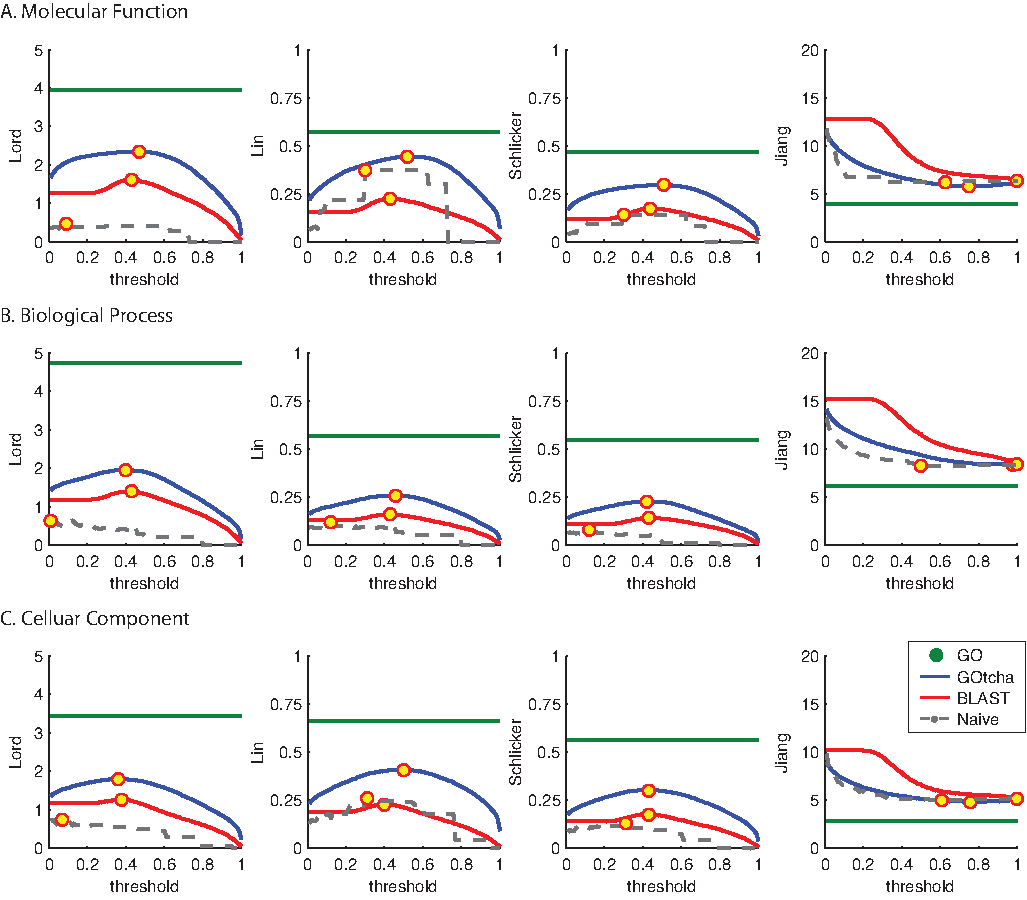
\includegraphics[width=\linewidth]{Figures/rumi/S1}
\par\end{centering}
\caption{Two-dimensional evaluation plots of information content-based metric performances when using the all-pair method of averaging. Yellow dots denote the maximum similarity or, in the case of  \citet{Jiang1997}, the minimum distance, that each method obtains.}
\end{figure*}


\begin{figure*}[h!]
\begin{centering}
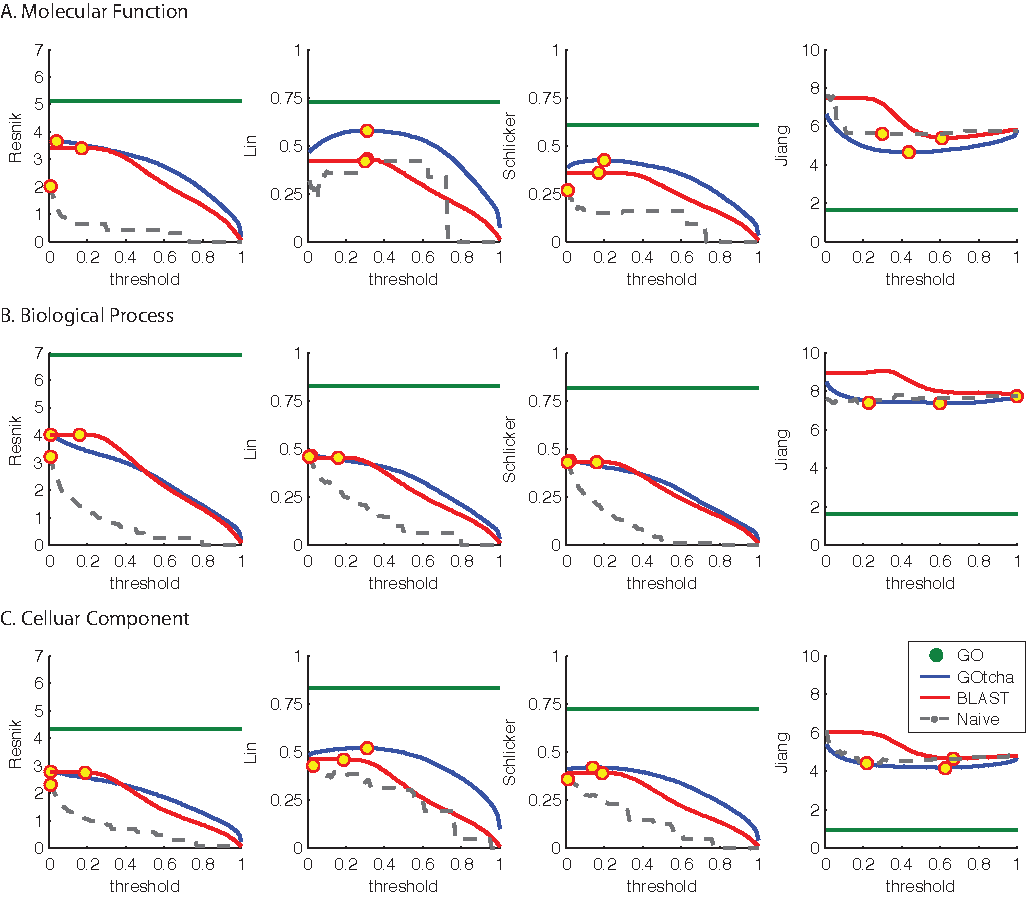
\includegraphics[width=\linewidth]{Figures/rumi/S2}
\par\end{centering}
\caption{Two-dimensional evaluation plots of information content-based metric performances when using the max-average method of averaging. Yellow dots denote the maximum similarity or, in the case of \citet{Jiang1997}, the minimum distance, that each method obtains.}
\end{figure*}

In Supplementary Figure 3 we contrast two different types of precision-recall curves. In the top row, we present the same results as in Figure 3 of the main manuscript. In the bottom row, we use precision-recall calculations according to \citet{Verspoor2006}. The methods provided similar results although the max-average formulation had generally larger values of $F_{\max}$ than the standard formulation of precision and recall (as defined in the main manuscript). However, these larger values of $F_{\max}$ occurred at lower decision thresholds.


\begin{figure*}[h!]
\begin{centering}
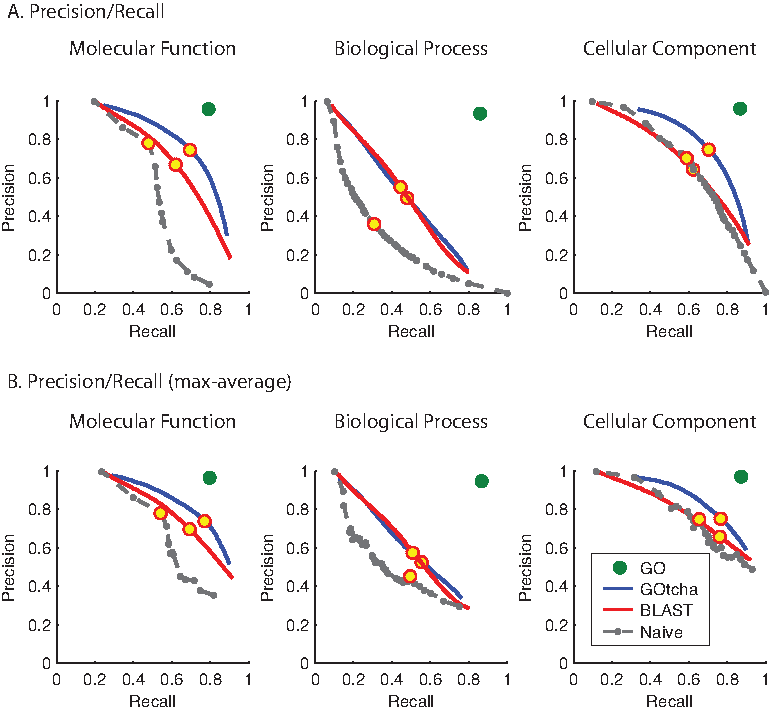
\includegraphics[width=\linewidth]{Figures/rumi/S3}
\par\end{centering}
\caption{Plots showing results using the standard method of calculating precision and recall (top row) compared to using the max-average method of calculating precision and recall as detailed by \citet{Verspoor2006} (bottom row). Yellow dots denote the values of precision and recall at which each method obtains its $F_{\max}$ value. }
\end{figure*}

In Supplementary Figure 4, we present more detailed results related to the ru-mi curves presented in Figure 3 of the main manuscript. In the top row, we show the same ru-mi curves as in the main manuscript, with yellow dots providing information where the maximum values of semantic distance $S_2$ were reached for each method. Interestingly, because the predictors generally associate scores to all nodes in the Gene Ontology, the amount of over-prediction can be very large for low decision thresholds, which consequently results in large values of misinformation. To provide better insight into the balance between remaining uncertainty and misinformation achieved by the semantic distance $S_2$, in the bottom row we present the same curves for small values of misinformation only.


\begin{figure*}[h!]
\begin{centering}
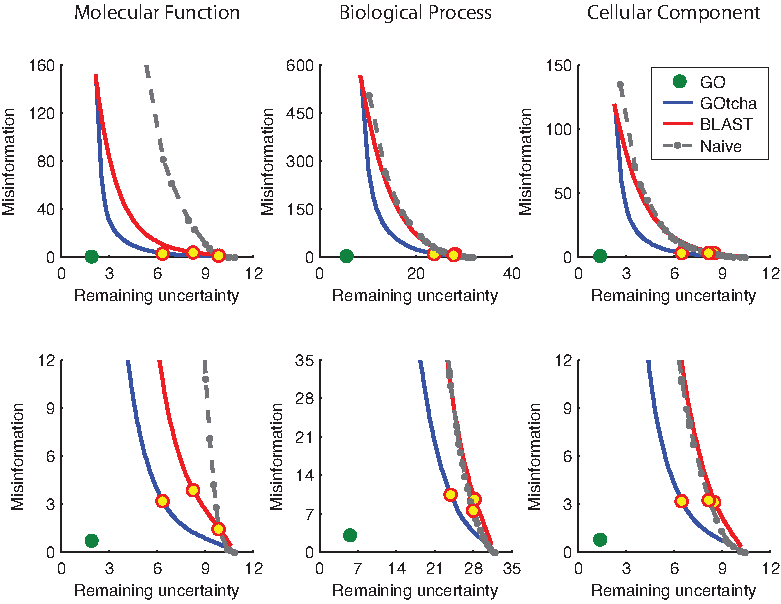
\includegraphics[width=\linewidth]{Figures/rumi/S4}
\par\end{centering}
\caption{Figures showing the remaining uncertainty and misinformation of baseline methods with yellow dots denoting values at which each method obtains its $S_{2}$ value. For better interpretation of the values at which each method achieves its $S_{2}$ value the bottom row of figures show the same plots as the top row, but with adjusted y-axis limits. }
\end{figure*}

%\clearpage
%\section{Supplemental tables}

Finally, in Supplementary Table 1, we provide results analogous to those from Table 1 in the main manuscript, but using max-average method instead of all-pair averaging. We generally observe similar trends as before, but note that the values of BLAST thresholds used for functional transfer are even lower than when all-pair averaging was used (except for the measure by \citealt{Jiang1997}, where max-average method seems to be beneficial). Therefore, we believe that, generally, all-pair averaging provides better results regarding functional similarity than does max-average.

\begin{table*}[h!]
\caption{Performance of information-theoretic methods when calculating performance as the average of maximum similarity (or distance) between each true and predicted term as described in Section \ref{sec:averaging}. The $F_{\max}$ values were calculated using the precision and recall according to \citet{Verspoor2006}. As in table Table 1 of the main manuscript, the decision threshold was varied across the entire range of predictions to obtain the maximum or minimum value (shown in column 1) for each method. The threshold at which each method reached the best value is shown in column 2. Columns 3 and 4 show the remaining uncertainty and misinformation calculated according to the Bayesian network. Each semantic similarity metric was calculated according to the relative frequencies of observing each term in the database.
\label{Tab:S01}}
\resizebox{\columnwidth}{!}
{\begin{tabular}{c|cccc|cccc|cccc}

\multicolumn{1}{l}{\hphantom} &\multicolumn{4}{c}{\bf Molecular Function } & \multicolumn{4}{c}{\bf Biological Process} &  \multicolumn{4}{c}{\bf Cellular Component } \\


\bf Resnik & Max & Threshold & RU & MI & Max & Threshold & RU & MI & Max & Threshold & RU & MI\\
\hline
\multicolumn{1}{l|}{GOtcha}& 3.65 & 0.04 & 2.96 & 32.17 & 4.02 & 0.01 & 10.19 & 273.90 & 2.80 & 0.01 & 2.70 & 59.02 \\
\multicolumn{1}{l|}{BLAST}& 3.41 & 0.17 & 2.17 & 151.77 & 4.03 & 0.16 & 8.48 & 566.88 & 2.77 & 0.19 & 2.26 & 119.34 \\
\multicolumn{1}{l|}{Naive}& 2.02 & 0.01 & 5.07 & 177.91 & 3.22 & 0.01 & 10.35 & 504.88 & 2.32 & 0.01 & 2.65 & 135.04 \\


\multicolumn{1}{l}{\hphantom} & & & &\multicolumn{1}{c}{\hphantom} & & & & \multicolumn{1}{c}{\hphantom} & & & &\\

\bf Lin & Max & Threshold & RU & MI & Max & Threshold & RU & MI & Max & Threshold & RU & MI\\
\hline
\multicolumn{1}{l|}{GOtcha}& 0.58 & 0.31 & 5.32 & 5.86 & 0.46 & 0.02 & 11.10 & 192.89 & 0.52 & 0.31 & 5.55 & 5.58 \\
\multicolumn{1}{l|}{BLAST}& 0.43 & 0.31 & 2.90 & 90.72 & 0.45 & 0.16 & 8.48 & 566.88 & 0.46 & 0.19 & 2.26 & 119.34 \\
\multicolumn{1}{l|}{Naive}& 0.42 & 0.30 & 10.39 & 0.21 & 0.46 & 0.01 & 10.35 & 504.88 & 0.43 & 0.03 & 3.90 & 56.83 \\


\multicolumn{1}{l}{\hphantom} & & & &\multicolumn{1}{c}{\hphantom} & & & & \multicolumn{1}{c}{\hphantom} & & & &\\

\bf Jiang & Min & Threshold & RU & MI & Min & Threshold & RU & MI & Min & Threshold & RU & MI\\
\hline
\multicolumn{1}{l|}{GOtcha}& 4.65 & 0.44 & 6.18 & 3.56 & 7.39 & 0.60 & 26.65 & 5.30 & 4.19 & 0.63 & 7.45 & 1.80 \\
\multicolumn{1}{l|}{BLAST}& 5.38 & 0.61 & 6.97 & 7.58 & 7.75 & 1.00 & 31.31 & 1.40 & 4.67 & 0.67 & 7.84 & 5.13 \\
\multicolumn{1}{l|}{Naive}& 5.61 & 0.30 & 10.39 & 0.21 & 7.41 & 0.23 & 27.73 & 8.49 & 4.45 & 0.22 & 8.17 & 3.25 \\


\multicolumn{1}{l}{\hphantom} & & & &\multicolumn{1}{c}{\hphantom} & & & & \multicolumn{1}{c}{\hphantom} & & & &\\

\bf Schlicker & Max & Threshold & RU & MI & Max & Threshold & RU & MI & Max & Threshold & RU & MI\\
\hline
\multicolumn{1}{l|}{GOtcha}& 0.42 & 0.20 & 4.56 & 9.32 & 0.44 & 0.02 & 11.10 & 192.89 & 0.42 & 0.14 & 4.29 & 12.76 \\
\multicolumn{1}{l|}{BLAST}& 0.36 & 0.17 & 2.17 & 151.77 & 0.43 & 0.16 & 8.48 & 566.88 & 0.39 & 0.19 & 2.26 & 119.34 \\
\multicolumn{1}{l|}{Naive}& 0.27 & 0.01 & 5.07 & 177.91 & 0.43 & 0.01 & 10.35 & 504.88 & 0.36 & 0.01 & 2.65 & 135.04 \\

\multicolumn{1}{l}{\hphantom} & & & &\multicolumn{1}{c}{\hphantom} & & & & \multicolumn{1}{c}{\hphantom} & & & &\\

$\mathbf{ F_{max} }$ & Max & Threshold & RU & MI & Max & Threshold & RU & MI & Max & Threshold & RU & MI\\
\hline
\multicolumn{1}{l|}{GOtcha}& 0.76 & 0.33 & 5.45 & 5.41 & 0.54 & 0.23 & 19.79 & 26.04 & 0.76 & 0.31 & 5.55 & 5.58 \\
\multicolumn{1}{l|}{BLAST}& 0.70 & 0.44 & 4.83 & 25.39 & 0.54 & 0.46 & 18.06 & 108.73 & 0.71 & 0.37 & 4.23 & 41.17 \\
\multicolumn{1}{l|}{Naive}& 0.64 & 0.29 & 9.87 & 1.44 & 0.47 & 0.07 & 22.06 & 51.55 & 0.70 & 0.20 & 7.23 & 6.75 \\


%\multicolumn{1}{l}{\hphantom} & & & &\multicolumn{1}{c}{\hphantom} & & & & \multicolumn{1}{c}{\hphantom} & & & &\\
\end{tabular}}{}
\end{table*}


